\section{Methodology\label{sec:assess.method}}

Assessing the impact of data-poisoning over \gls{fl} implies reviewing a consequent amount of parameters and configurations.
To optimize our work and make it easily reproducible, the results presented in \Cref{sec:assess.results} have been generated using a purposely designed evaluation framework based on Flower~\cite{beutel_Flowerfriendlyfederated_2020} and Hydra~\cite{Hydra}.
We follow the ACM's guidelines and terminology~\cite{ACM_artifacts}, and take measures to ensure the \emph{reusability} of our artifacts, the \emph{reproducibility} of our results, and the \emph{replicability} of our experiments.
Specifically:
\begin{enumerate}[1.]
    \item We provide the methodology and all parameters necessary to reimplement and replicate the experiments;
    \item Dependencies are pinned using Poetry for Python and Nix for system, allowing the entire software pipeline to be executed in the same conditions;
    \item All experiments are seeded where possible, which makes the results reproducible within a three decimal precision;
    \item The results and the code to generate them are available in open access\footnote{\codeurl}, as are the datasets\footnote{\url{https://staff.itee.uq.edu.au/marius/NIDS_datasets/}}.
\end{enumerate}

The results presented in this paper amount to 10~670 unique runs, and close to 1~613 cumulated computing hours on two NixOS servers with 96 cores, 768~GB of RAM and 2 Nvidia Tesla T4 each. 



\subsection{Dataset and Pre-processing\label{sec:assess.method.dataset}}

\begin{figure}
  \begin{subfigure}{.45\linewidth}
    \centering
    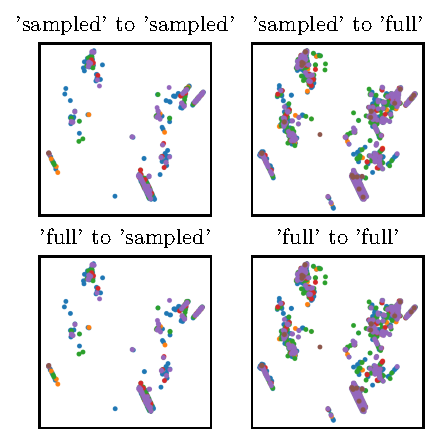
\includegraphics{figures/cicids/pca-projection.pdf}
    \caption{CIC-CSE-IDS2018\label{fig:assess.pca.cicids}}
  \end{subfigure}
  \hfill
  \begin{subfigure}{.45\linewidth}
    \centering
    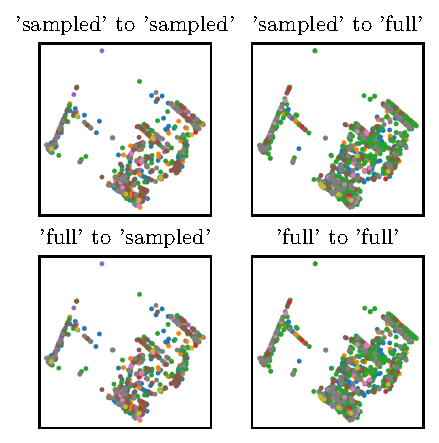
\includegraphics{figures/nb15/pca-projection.pdf}
    \caption{UNSW-NB15\label{fig:assess.pca.nb15}}
  \end{subfigure}
  \caption[
    Cross-projections of the malicious traffic from the two datasets in 2D using \gls{pca}.
  ]{
    Cross-projections of the malicious traffic from the two datasets in 2D using \gls{pca}.
    On top, the frame of reference is computed using the \texttt{sampled} dataset, and on the bottom the \texttt{full} dataset.
    The \texttt{sampled} dataset is then projected on the left, the \texttt{full} dataset on the right.
    }
  \label{fig:assess.pca}
\end{figure}

\begin{table}
  \centering
  \caption{
    Distribution of the CIC-CSE-IDS2018 and UNSW-NB15 (NF-V2) datasets~\cite{sarhan_StandardFeatureSet_2022,layeghy_GeneralisabilityMachineLearningbased_2022}.
    \label{tbl:assess.datasets}
  }
  \hfill
\begin{minipage}{.48\textwidth}
  \small
  \begin{tabularx}{\linewidth}{lXrr}
    \toprule % ------------------------------------
    \multicolumn{1}{c}{\textbf{Class}} & & \multicolumn{1}{c}{\textbf{Sampled}} & \multicolumn{1}{c}{\textbf{Full}} \\
    \midrule % ---------------------------------
    Benign         & & 880,623   & 16,635,567 \\
    DDoS           & & 73,558    & 1,390,270  \\
    DoS            & & 25,574    & 483,999    \\
    Bot            & & 7,595     & 143,097    \\
    Brute Force    & & 6,525     & 123,982    \\
    Infiltration   & & 6,108     & 116,361    \\
    Injection      & & 17        & 432        \\
    & & & \\
    & & & \\
    & & & \\
    \midrule % ---------------------------------
    \textbf{Total} & & 1,000,000 & 18,893,708 \\
    \bottomrule % ---------------------------------
  \end{tabularx}
\end{minipage}
\hfill
\begin{minipage}{.48\textwidth}
  \small
  \begin{tabularx}{\linewidth}{lXrr}
    \toprule % ---------------------------------
    \multicolumn{1}{c}{\textbf{Class}} & & \multicolumn{1}{c}{\textbf{Sampled}} & \multicolumn{1}{c}{\textbf{Full}} \\
    \midrule % ---------------------------------
    Benign           & & 960,078  & 2,295,222   \\
    Exploits         & & 13,187   & 31,551      \\
    Fuzzers          & & 9,377    & 22,310      \\
    Generic          & & 6,976    & 16,560      \\
    Reconnaissance   & & 5,352    & 12,779      \\
    DoS              & & 2,455    & 5,794       \\
    Analysis         & & 969      & 2,299       \\
    Backdoor         & & 925      & 2,169       \\
    Shellcode        & & 617      & 1,427       \\
    Worms            & & 64       & 164         \\
    \midrule % ---------------------------------
    \textbf{Total}   & & 1,000,000 & 2,390,275  \\
    \bottomrule % ------------------------------
  \end{tabularx}
\end{minipage}
\hfill
\end{table}



Due to the scale of the required experiments, we require a datasets that are both representative of the problem and small enough to be processed in a reasonable amount of time.
As discussed in \Cref{chap:background,chap:application}, recent works on \gls{fl} and \gls{ids}~\cite{sarhan_StandardFeatureSet_2021} proposed a standardized feature set (NF-V2) making cross-dataset \gls{fl} setups easier.
The authors notably provide converted versions of known datasets, including CSE-CIC-IDS2018~\cite{sharafaldin_GeneratingNewIntrusion_2018} and UNSW-NB15~\cite{moustafa_UNSWNB15comprehensivedata_2015}, the two most used generic \gls{nids} datasets in the literature.

Due to the scale of the required experiments, we use the ``sampled'' version of the datasets provided by the authors~\cite{layeghy_GeneralisabilityMachineLearningbased_2022}, and already mentioned in \Cref{chap:application}.
After pre-processing, we evenly split the dataset for the experiments, ensuring the same class distribution in the training and testing sets.
80\% of the dataset is used for training, and 20\% for testing.
We purposely do not use a proper validation set, as the goal is to measure the performance delta related to the impact of the attacks on the global model, and not to optimize the model's hyperparameters.
Indeed, the parameters are kept constant throughout the experiments, as detailed in \Cref{tbl:hyperparams}.
We sometimes refer to the datasets as \texttt{cicids} and \texttt{nb15} for brevity in the remaining of this chapter.

To assess the representativity of the datasets sampling, we compare the projections in two dimensions of the two datasets using \gls{pca}.
\Cref{fig:assess.pca} presents cross-projections results, depending on the datasets used to generate the projection frame.
There are consequent overlaps between the classes in this projection, implying that either 2 dimensions are not enough to separate the classes, or there are features that are not relevant to the classification task.
Yet, the projected patterns are identical between the two datasets, which indicates that the sampling process does not introduce significant distribution bias in the dataset.
Therefore, experiments performed over the sampled datasets should be representative of observed the behaviors in the original dataset.


\subsection{Local and Federated Training\label{sec:assess.method.models}}

%\begin{wraptable}{L}{.4\linewidth}
\begin{table}
  \newcommand{\cellcenter}[1]{\multicolumn{1}{c}{#1}}
  \centering
  \caption{Hyperparameters.\label{tbl:hyperparams}}
  \small
  \begin{tabular}{ll}
    \toprule % ------------------------------------
    \cellcenter{\textbf{Hyperparameter}}   & \cellcenter{\textbf{Value}} \\
    \midrule % ---------------------------------
    Learning rate             & 0.0001 \\
    Hidden layers activation  & ReLU \\
    Output layer activation   & Sigmoid \\
    Input shape               & 49 \\
    Number of hidden layers   & 2 \\ 
    Size of the hidden layers & 128 \\
    Optimizer                 & Adam \\
    Loss function             & Binary cross-entropy \\
    % Loss function             & Log loss \\
    %                          & (binary cross-entropy) \\
    Aggregation               & \texttt{FedAvg} \\
    \bottomrule % ---------------------------------
  \end{tabular}
\end{table}
%\end{wraptable}

We use a simple \gls{mlp} model with two hidden layers, as implemented by \textcite{popoola_FederatedDeepLearning_2021} who use the same datasets; a summary of the model's parameters is available in \Cref{tbl:hyperparams}.
Trained centrally, this model reaches an F1-score of 0.966 and an accuracy of 0.992 on our sampled CIC-CSE-IDS2018, and 0.945 and 0.995 on the UNSW-NB15 dataset, respectively.
These values can be considered as baselines for the \gls{fl} experiments.
% TODO: The scores are taken from the experiments made on Trust-FIDS; we should recompute them using this repo's version.
% exp info
% - repo: https://gitlab.imt-atlantique.fr/l20lavau/trust-fids/
% - commit: 88d7c3f95f2186c7ca6dbe61d927a4c33ff25317
% - tag: data-assessment
% - path: exps/results/popoola_mlp.ipynb

We focus on the impact of data-poisoning specifically, and therefore omit other factors that could hurt the performance of the model, such as client heterogeneity or disconnections.
We also specifically concentrate our efforts on a collaborative cross-silo setting, where all clients are available at each round and $C=1$.
Consequently, the dataset is partitioned into 10 \gls{iid} shards of 80,000 data points, and each client is assigned with one shard.
On the server, the uploaded models are aggregated using \texttt{FedAvg}---which, since the local datasets are of similar size, is equivalent to a simple average of the weights.

\subsection{Attack Model and Implementation\label{sec:assess.method.poisoning}}

We consider data-poisoning attacks where malicious participants can alter their local datasets before training.
This definition covers both, participants that have been compromised and those that are deliberately modifying their data.
Further, this scenario will always be available, even with a secure and immutable \gls{fl} client software.
Specifically, we implement data-poisoning using label-flipping attacks, where the attacker changes the label $y$ of a sample to a new label $y_p$; \ie, $y_p = \neg y$ in a binary-classification problem.

\paragraph{Attacker's Objective}

We consider two types of objectives for the attacker depending on the type of attack leveraged.
With \emph{targeted} attacks, the attacker aims to make a specific attack pattern undetectable, and therefore act as a backdoor in the \gls{ids}.
This is implemented by labeling a randomly selected fraction of a specific attack class (\eg, \emph{DDoS}) as benign.
With \emph{untargeted} attacks, on the other hand, his goal is to produce high \gls{fpr} and \gls{fnr}, which can overwhelm human operators or other security systems.
Here, a random fraction of the entire dataset is altered, where the label of each sample is flipped from benign to attack and vice versa.
The proportion of samples that are altered is controlled by the \gls{dpr}, which is the ratio of samples matching the target that are altered by each attacker on a specific round.
We note the \gls{dpr}, or \emph{local poisoning rate}, as $\alpha$.


\paragraph{Attacker's Knowledge and Capabilities}

We consider attackers to be \emph{gray-box} adversaries, \ie, they have the same knowledge as benign clients, but are unable to modify the system's behavior, neither locally nor on the server.  
Further, we consider that multiple attackers can be present in the system, and that they can act in concert. 
This scenario is referred to as \emph{colluding attackers}.
In this case, the attackers share the same target and \gls{dpr}.
The proportion of attackers can vary from one single malicious client to a majority of them being malicious, and is expressed as $\tau$, or \gls{mpr}~\cite{merzouk_Parameterizingpoisoningattacks_2023}.
Note that in the context of \gls{iid} partitioning, the overall poisoning rate could be regarded as $\alpha \times \tau$.
This simplification is however not accurate in other partitioning strategies.


\subsection{Experiments\label{sec:assess.method.exps}}

\begin{table}
  % LTeX: enable=false
    \centering
    \caption{Experimental parameters. Default parameters are highlighted in bold and are used if not specified otherwise.}
    \label{tbl:expsparams}
    \footnotesize
    \setlength{\extrarowheight}{3pt}
    \begin{tabular}{>{\ttfamily\itshape}p{.12\linewidth} >{\ttfamily}p{.8\linewidth}}
      \toprule
      \normalfont{\textbf{Parameter}} & \normalfont{\textbf{Values}} \\
      \midrule
      dataset      & cicids, nb15                                                                                                                                                                                \\
      batch\_size  & 32, 128, \textbf{512}                                                                                                                                                                       \\
      epochs       & \textbf{100\_10x10}, 100\_4x25, 100\_1x100, 300\_10x30, 300\_4x75, 300\_1x300                                                                                                               \\
      distribution & 10-0, 9-1, 7-3, \textbf{5-5}, 3-7                                                                                                                                                           \\
      scenario     & continuous-\{10,30,60,70,80,90,95,99\}, \textbf{continuous-100}, late-3, redemption-3                                                                                                       \\
      target       & \textbf{untargeted}, (cicids) bot, dos, ddos, bruteforce, infiltration, injection, (nb15) generic, analysis, worms, backdoor, exploits, untargeted, shellcode, dos, reconnaissance, fuzzers \\
      partitioner  &  iid\_drop\_1, iid\_drop\_2, \textbf{iid\_full}, iid\_keep\_1, kmeans\_drop\_1, kmeans\_drop\_2, kmeans\_full, kmeans\_keep\_1                                                              \\
      seed         & 1313, 1977, 327, 5555, 501, 421, 3263827, 2187, 1138, 6567                                                                                                                                  \\
      \bottomrule
    \end{tabular}
  % LTeX: enable=true
  \end{table}

We design a set of experiments to answer the research questions laid out in \Cref{sec:assess.intro}.
All experiments share a common set of constants, which are complemented by a set of variable parameters.
\Cref{tbl:expsparams} summaries the available parameters for the experiments.
Each combination is tested 10 times using a set of 10 different seeds to study the predictability of the results.
Specifically, the seed impacts data-partitioning operations (both between the training and testing sets, and among clients afterward), the sample selection in poisoning attacks, and the random weights of the initial model. It also impacts all the random operations (such as data shuffling) done during model training.

The \texttt{epochs} parameter controls the aggregation frequency, \ie, the number of local epochs per round $\mathcal{E}$, as well as the number of rounds $R$.
Logically, \texttt{batch\_size} controls the size of the batches used at each iteration during training.
The global number of local epochs per client is kept to 100 or 300 to preserve comparability.
The \texttt{distribution} represents the number of legitimate and malicious clients in the system, and consequently the proportion of attackers.
The key \texttt{scenario} represents the attackers' behavior. 
Scenarios defined as $\texttt{continuous-}\alpha$ represent a constant poisoning rate of $\alpha$ over the entire training process.
Scenarios named $\texttt{late-}r$ and $\texttt{redemption-}r$ produce an attack with $\alpha=100$ that starts or ends at round $r$, respectively.
Parameter \texttt{target} represents the target of the attack as defined in \Cref{sec:assess.method.poisoning}; each attack class is made available as a target. 


\subsubsection{Partitioning Strategies\label{sec:assess.method.partition}}

\begin{figure}
  \centering
  \begin{subfigure}{.49\linewidth}
    \centering
    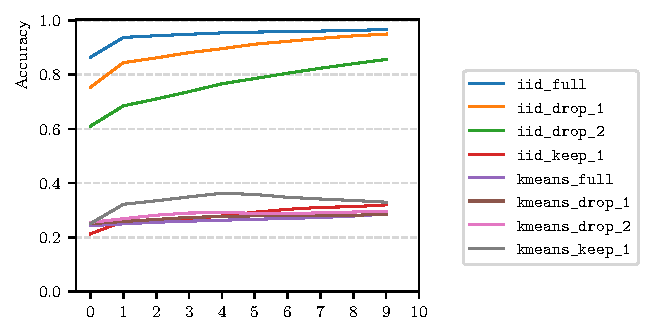
\includegraphics[width=\linewidth]{figures/cicids/niid-perf.pdf}
    \caption{CIC-CSE-IDS2018\label{fig:assess.niid.cicids}}
  \end{subfigure}
  \hfill
  \begin{subfigure}{.49\linewidth}
    \centering
    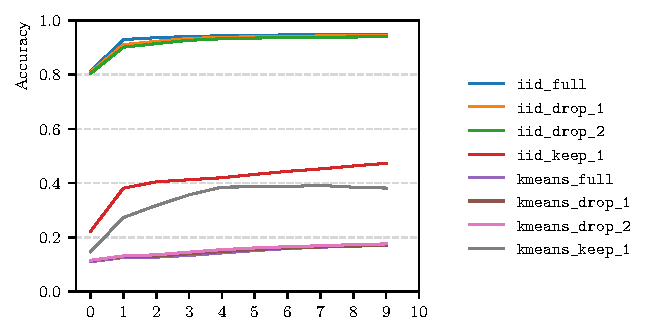
\includegraphics[width=\linewidth]{figures/nb15/niid-perf.pdf}
    \caption{UNSW-NB15\label{fig:assess.niid.nb15}}
  \end{subfigure}
  \caption{
    Impact of the partitioning strategy on the model's performance.
    \label{fig:assess.niid}
  }
\end{figure}

A particular parameter in this selection is the \texttt{partitioner}, which defines the strategy used to partition the dataset among the clients.
As mentioned in \Cref{sec:app.demo.setup}, the literature of \glspl{fids} usually considers either \gls{iid} partitioning or basic \gls{niid} scenarios where clients randomly drop attack classes.
To study the usage of similarity metrics to detect poisoning attacks, we consider eight different partitioning strategies, with different levels of heterogeneity that range from \gls{iid} partitioning to \emph{pathological}\footnotemark{} settings without distribution overlap.

\footnotetext{{Refers to the \emph{pathological} \gls{niid} partitioning~\cite{mcmahan_Communicationefficientlearningdeep_2017} discussed in \Cref{chap:background}.}}

The \texttt{partitioners} marked named \texttt{iid\_*} distribute the data in an \gls{iid} manner, where each client receives a stratified\footnotemark{} subset of the dataset.
Then, \texttt{full}, \texttt{drop\_*}, and \texttt{keep\_*} refer to the way the attack classes are processed: all kept, certain classes dropped, or certain classes kept, respectively.
The \texttt{kmeans\_*} partitioners use a $k$-means clustering algorithm to partition the benign traffic among the clients, and then distribute the attack classes based on their attribute (\texttt{full}, \texttt{drop\_*}, \texttt{keep\_*}).
Because $k$-means algorithm minimizes the intra-cluster variance, it increases the heterogeneity of the clients' datasets.
\Cref{fig:assess.niid} illustrates performance of the model under different partitioning strategies.

\footnotetext{
  Stratified sampling ensures that the class distribution remains the same among the different shards.
  It is usually done using the labels of the samples, but any categorical feature can be used.
}


\subsection{Metrics\label{sec:assess.method.metrics}}

To quantify how the experiment parameters impact the global model, we define a set of metrics to measure the \gls{asr} of poisoning attacks.
The definition of the \gls{asr} differs depending on the type of attack, according to the attacker's objective defined in \Cref{sec:assess.method.poisoning}.
Because the \gls{asr} is based on performance and that no perfect model exists, we distinguish the \gls{aasr} measured on the attack scenario, from the \gls{rasr} which also considers the nominal performance without attacks.
Formally, the \gls{rasr} is defined as:

\begin{equation}
  \label{eq:rasr}
  % rasr = ((np.maximum(ref, aasr) - ref) / (1 - ref)).astype(float)
  \text{RASR} = \frac
    {\max(\text{AASR}_{benign}, \text{AASR}_{attack}) - \text{AASR}_{benign}}
    {1 - \text{AASR}_{benign}},
\end{equation}

where $\text{AASR}_{benign}$ and $\text{AASR}_{attack}$ are the \gls{aasr} of the \emph{benign} and \emph{attack} scenarios respectively, under the same set of parameters. 
This is made possible thanks to the framework's reproducibility, which ensures two experiments started with the same seed will run under the same conditions.
Following the definitions in \Cref{sec:assess.method.poisoning}, we then defined two variations of the \gls{aasr} depending on the attacker's objective.
Both are computed based on the confusion matrix of the model: \gls{tp}, \gls{tn}, \gls{fp}, and \gls{tn}.

\begin{description}[font=\normalfont\textit]
  \item[Targeted attacks:]
    Malicious participants leverage targeted attacks to make a specific attack pattern undetectable.
    Therefore, a successful attack forces classification of the relevant attack samples as benign.
    The \gls{aasr} is then defined as the miss rate of the targeted attack, \ie

    \begin{equation}
      \label{eq:aasr_targeted}
      \text{AASR} = \frac
        {\text{FN}_c}
        {\text{TP}_c + \text{FN}_c},
    \end{equation}

    where $c$ is a specific attack class of the dataset.

  \item[Untargeted Attacks:]
    Untargeted attacks aim at degrading the overall classification rate of the model.
    Consequently, the \gls{aasr} is defined as the miss-classification rate of the model, \ie

    \begin{equation}
      \label{eq:aasr_untargeted}
      \text{AASR} = \frac
        {\text{FP} + \text{FN}}
        {\text{TP} + \text{TN} + \text{FP} + \text{FN}}
        = 1 - \text{accuracy}.
    \end{equation}
\end{description}

Additionally, we use traditional binary classification metrics to observe the performance of the model under various conditions, as identified in existing surveys~\cite{campos_EvaluatingFederatedLearning_2022,lavaur_EvolutionFederatedLearningbased_2022}
These metrics include \emph{accuracy}, \emph{F1-score}, and \emph{miss rate}.
Notably, we consider the \gls{mta}, defined as the accuracy of the benign clients obtained on the testing set, to measure the impact of the attacks on the model's nominal performance.
All metrics are aggregated over the 10 runs of each experiment, and the mean and standard deviation are reported for the selected metric.